% =============================================================================
%  Fermiony Majorany i ich realizacja w nanodrutach półprzewodnikowych
%  Materiały i przyrządy półprzewodnikowe — prezentacja (pierwszy szkic)
%
%  Kompilacja: make   (latexmk -lualatex)
%  Wykresy własne: python3 sim/wykresy.py  ->  fig/*.pdf
%  Rysunki z [LF12] (Leijnse & Flensberg 2012): fig/ref/rys{1,3,4,5}.png
%
%  Podział:  Prelegent A — slajdy 1–22 (~28 min)
%            Prelegent B — slajdy 23–42 (~27 min)
%  Znacznik \sprawdz{...} = fakt/liczba do weryfikacji przed wystąpieniem.
% =============================================================================
\documentclass[aspectratio=169,10pt]{beamer}

\usetheme[progressbar=frametitle,numbering=fraction,sectionpage=none,block=fill]{metropolis}
\usefonttheme{serif}
\usefonttheme{professionalfonts}

\usepackage{amsmath}
\usepackage{mathtools}
\usepackage{fontspec}
\usepackage{unicode-math}
\setmainfont{STIX Two Text}
\setsansfont{STIX Two Text}
\setmathfont{STIX Two Math}
\setmonofont{JetBrains Mono}[Scale=MatchLowercase]
\usepackage{braket}
\usepackage[polish]{babel}
\usepackage{luavlna}
\singlechars{polish}{AaIiOoUuWwZz}
\usepackage{microtype}
\usepackage{newunicodechar}
% STIX Two Text nie ma tych znaków — bierzemy je z fontu matematycznego
\newunicodechar{→}{\ensuremath{\rightarrow}}
\newunicodechar{⇒}{\ensuremath{\Rightarrow}}
\newunicodechar{≈}{\ensuremath{\approx}}
\usepackage{csquotes}
\DeclareQuoteAlias[guillemets*]{polish}{polish}
\usepackage{graphicx}
\usepackage{booktabs}
\usepackage{tabularx}
\usepackage{xcolor}
\usepackage{siunitx}
\sisetup{
    per-mode=symbol,
    exponent-product=\times,
    range-units=repeat,
    output-decimal-marker={.}
}
\usepackage{listings}
\lstset{
    basicstyle=\ttfamily\scriptsize,
    language=Python,
    breaklines=false,
    frame=single,
    columns=fullflexible,
    keywordstyle=\color{mBlue}\bfseries,
    commentstyle=\color{gray}
}
\usepackage{appendixnumberbeamer}
\usepackage{tikz}
\usetikzlibrary{arrows.meta, positioning, calc, decorations.pathmorphing, babel}

\DeclarePairedDelimiter\abs{\lvert}{\rvert}
\AtBeginDocument{
    \let\square\mdlgwhtsquare
    \let\blacksquare\mdlgblksquare
    \let\varpropto\propto
}

% --- kolory (zgodne z wykresami z sim/wykresy.py) ----------------------------
\definecolor{mBlue}{HTML}{1F5FA8}
\definecolor{mRed}{HTML}{C8323C}
\definecolor{mGreen}{HTML}{2A8A4A}
\definecolor{mDark}{HTML}{1E2A3A}
\setbeamercolor{frametitle}{bg=mDark}
\setbeamercolor{progress bar}{fg=mRed, bg=mDark!30}
\setbeamercolor{alerted text}{fg=mRed}
\setbeamercolor{block title}{bg=mBlue!15, fg=mDark}
\setbeamercolor{block body}{bg=mBlue!5}

% --- makra pomocnicze ---------------------------------------------------------
\newcommand{\prelegent}{cz.\,I — Prelegent A}
\setbeamertemplate{frame footer}{Fermiony Majorany w nanodrutach \quad·\quad \prelegent}
% źródło rysunku/danych w prawym dolnym rogu slajdu
\newcommand{\zrodlo}[1]{%
  \begin{tikzpicture}[remember picture, overlay]
    \node[anchor=south east, font=\tiny, text=gray, align=right, text width=13cm]
      at ([xshift=-3mm, yshift=6.5mm]current page.south east) {#1};
  \end{tikzpicture}}
% znacznik „do weryfikacji” — usunąć w wersji końcowej
\newcommand{\sprawdz}[1][sprawdzić]{\textcolor{mRed}{\scriptsize\,[#1]}}
\newcommand{\LF}{[LF12]}
\newcommand{\hc}{\mathrm{h.c.}}
\newcommand{\eV}{\unit{\electronvolt}}

% =============================================================================
\title{Fermiony Majorany i ich realizacja\\ w nanodrutach półprzewodnikowych}
\subtitle{Materiały i przyrządy półprzewodnikowe}
\author{Prelegent A \and Prelegent B} % TODO: imiona i nazwiska
\date{\today}                          % TODO: data wystąpienia
\institute{}

\begin{document}

% =============================================================================
%  CZĘŚĆ I — Prelegent A (slajdy 1–22, ~28 min)
% =============================================================================

% --- 1 ----------------------------------------------------------------------
\begin{frame}[plain]
  \titlepage
\end{frame}

% =============================================================================
\section{Motywacja}
% =============================================================================

% --- 2 (~2 min) --------------------------------------------------------------
\begin{frame}{Dlaczego Majorany? Problem dekoherencji}
  \begin{itemize}
    \item Kubit fizyczny (spin, ładunek, strumień) przechowuje informację
          \alert{lokalnie} → każde lokalne zaburzenie (fluktuacje ładunku,
          pola, fonony) może ją zmienić lub „podejrzeć”.
    \item Pomysł Kitaeva (2001): zapisać bit w obsadzeniu fermionu
          rozdzielonego na dwie \alert{odległe połówki} $\gamma_1$, $\gamma_2$.
    \item Lokalny szum „widzi” tylko jedną połówkę — nie może ani odczytać,
          ani zmienić stanu. Błędy tłumione jak $e^{-L/\xi}$:
          ochrona \alert{sprzętowa}, nie programowa.
  \end{itemize}
  \vspace{1mm}
  \centering
  \begin{tikzpicture}[scale=0.92]
    \fill[mBlue!25] (0,0.5) rectangle (8,0.72);
    \shade[left color=gray!45, right color=gray!65, rounded corners=3pt] (0,0) rectangle (8,0.5);
    \node[font=\tiny] at (4,0.61) {nadprzewodnik (Al)};
    \node[font=\scriptsize, white] at (4,0.25) {nanodrut};
    \fill[mRed] (0.35,0.25) circle (0.13);
    \fill[mRed] (7.65,0.25) circle (0.13);
    \node[below=1pt] at (0.35,0) {$\gamma_1$};
    \node[below=1pt] at (7.65,0) {$\gamma_2$};
    \draw[dashed, thick, mBlue] (0.35,0.75) .. controls (2,1.9) and (6,1.9) .. (7.65,0.75);
    \node[mBlue, font=\small] at (4,1.75) {$c=\tfrac12(\gamma_1+i\gamma_2)$ — jeden nielokalny stan};
    \draw[-{Stealth}, very thick, orange!90!black, decorate,
          decoration={zigzag, segment length=4pt, amplitude=1.5pt, post length=3pt}]
          (-1.3,1.3) -- (0.15,0.45);
    \node[font=\scriptsize, align=center] at (-1.5,1.65) {lokalny szum};
    \draw[{Stealth}-{Stealth}] (0.35,-0.55) -- node[fill=white, font=\scriptsize] {$L\gg\xi$} (7.65,-0.55);
  \end{tikzpicture}
\end{frame}

% --- 3 (~2 min) --------------------------------------------------------------
\newcommand{\tlup}[3]{%
  \fill[mRed] (#1,0) circle (2.3pt);
  \node[below=3pt, font=\scriptsize\bfseries] at (#1,0) {#2};
  \draw[gray] (#1,0.08) -- (#1,0.35);
  \node[above, text width=2.3cm, align=center, font=\scriptsize] at (#1,0.35) {#3};}
\newcommand{\tldown}[3]{%
  \fill[mRed] (#1,0) circle (2.3pt);
  \node[above=3pt, font=\scriptsize\bfseries] at (#1,0) {#2};
  \draw[gray] (#1,-0.08) -- (#1,-0.35);
  \node[below, text width=2.3cm, align=center, font=\scriptsize] at (#1,-0.35) {#3};}
\begin{frame}{Oś czasu}
  \centering
  \begin{tikzpicture}[x=1.43cm]
    \draw[very thick, -{Stealth}, mDark] (-0.4,0) -- (8.55,0);
    \tlup{0}{1937}{Majorana: rzeczywiste rozwiązania równania Diraca}
    \tldown{1}{2001}{Kitaev: łańcuch p-wave, mody zerowe na końcach}
    \tlup{2}{2010}{Lutchyn–Sau–Das Sarma, Oreg–Refael–von Oppen: przepis z~nanodrutem}
    \tldown{3}{2012}{Delft (Mourik i in.): pik przy zerowym napięciu}
    \tlup{4}{2015}{epitaksjalny Al: twarda przerwa (Krogstrup, Chang)}
    \tldown{5}{2018→21}{„kwantyzacja $2e^2/h$” (Zhang i in.) — \alert{retrakcja}}
    \tlup{6}{2023}{Microsoft: TGP; Delft: minimalny łańcuch Kitaeva z~kropek}
    \tldown{7}{2025}{Microsoft: pomiar parzystości (Nature), tetron, „Majorana~1”}
    \tlup{8}{2026}{„Majorana~2” (Pb), spór o~TGP i odczyt $C_Q$ \sprawdz}
  \end{tikzpicture}
\end{frame}

% =============================================================================
\section{Majorana w ciele stałym}
% =============================================================================

% --- 4 (~1.5 min) ------------------------------------------------------------
\begin{frame}{Operator Majorany — „połowa” fermionu}
  \begin{columns}[T]
    \begin{column}{0.48\textwidth}
      Dowolny fermion $c$ rozkładamy na część „rzeczywistą” i~„urojoną”:
      \begin{align*}
        \gamma_1 &= c^\dagger + c, \qquad \gamma_2 = i\,(c^\dagger - c),\\
        c &= \tfrac12(\gamma_1 + i\gamma_2).
      \end{align*}
      Własności:
      \[
        \gamma_j = \gamma_j^\dagger,\qquad \gamma_j^2 = 1,\qquad
        \{\gamma_i,\gamma_j\} = 2\delta_{ij}.
      \]
    \end{column}
    \begin{column}{0.48\textwidth}
      \begin{itemize}
        \item Cząstka = własna antycząstka (w~ciele stałym: \alert{własna dziura}).
        \item „Liczba obsadzeń” $\gamma^\dagger\gamma = 1$ — pojedynczy
              Majorana \alert{nie ma} stanu; stan niesie dopiero para:
              \[ n = c^\dagger c = \tfrac12\,(1 + i\gamma_1\gamma_2). \]
        \item Rozkład jest zawsze możliwy, ale trywialny, gdy $\gamma_1$, $\gamma_2$
              siedzą w~tym samym miejscu. Fizyka zaczyna się, gdy są
              \alert{przestrzennie rozdzielone}.
      \end{itemize}
    \end{column}
  \end{columns}
  \zrodlo{\LF{} równ.~(2)–(5), (12)–(15)}
\end{frame}

% --- 5 (~1 min) --------------------------------------------------------------
\begin{frame}{Kwazicząstki Bogoliubowa: elektron + dziura}
  \begin{itemize}
    \item W~nadprzewodniku wzbudzenia są superpozycjami elektronu i~dziury.
    \item Nadprzewodnik \alert{s-wave} (singlet): pary $\uparrow\downarrow$
          \[ b = u\,c^\dagger_\uparrow + v\,c_\downarrow \quad\Rightarrow\quad b\neq b^\dagger \]
          (elektron i~dziura o~\emph{przeciwnych} spinach — to nie Majorana).
    \item Majorana wymaga równej wagi elektronu i~dziury \alert{o~tym samym spinie}:
          \[ \gamma = u\,c^\dagger_\sigma + u^*c_\sigma = \gamma^\dagger. \]
    \item Parowanie identycznych fermionów → zakaz Pauliego wymusza
          nieparzystą część orbitalną: $\Delta(k)\propto k$ — \alert{„bezspinowe” p-wave}.
    \item Naturalnych nadprzewodników p-wave praktycznie nie znamy
          → trzeba je \alert{zbudować} z~dostępnych składników.
  \end{itemize}
  \zrodlo{\LF{} rozdz.~1}
\end{frame}

% --- 6 (~1.5 min) ------------------------------------------------------------
\begin{frame}{Symetria cząstka–dziura i mody zerowe}
  \begin{columns}[T]
    \begin{column}{0.5\textwidth}
      Opis Bogoliubowa–de Gennesa (BdG) w~bazie Nambu
      \[
        \bar\Psi = \bigl(\Psi_\uparrow,\ \Psi_\downarrow,\ \Psi^\dagger_\downarrow,\ -\Psi^\dagger_\uparrow\bigr)^T
      \]
      Podwojenie bazy → symetria
      \[
        \mathcal{P} = \tau_y\otimes\sigma_y\,K,\qquad
        \mathcal{P}\,H_\mathrm{BdG}\,\mathcal{P}^\dagger = -H_\mathrm{BdG}.
      \]
      Stany występują parami: $E \leftrightarrow -E$, \ $\Psi_{-E} = \Psi_E^\dagger$.
    \end{column}
    \begin{column}{0.46\textwidth}
      \begin{block}{Wniosek}
        Majorana: $\Psi = \Psi^\dagger$ $\Rightarrow$ $E = -E$ $\Rightarrow$
        \alert{$E = 0$}.
        \[
          \bar\psi_M(\mathbf r) = \bigl(f,\ g,\ g^*,\ -f^*\bigr)^T
        \]
      \end{block}
      \begin{itemize}
        \item Izolowany mod zerowy nie może opuścić $E=0$ w~sposób ciągły —
              potrzebuje partnera.
        \item Szczegóły BdG: slajd zapasowy.
      \end{itemize}
    \end{column}
  \end{columns}
  \zrodlo{\LF{} równ.~(36)–(48)}
\end{frame}

% --- 7 (~1 min) --------------------------------------------------------------
\begin{frame}{Dlaczego potrzebne pole magnetyczne — argument Kramersa}
  \begin{itemize}
    \item Jeżeli $H$ jest symetryczny względem odwrócenia czasu,
          $\mathcal{T} = i\,\tau_0\otimes\sigma_y K$, \ $\mathcal{T}^2 = -1$,
          to każdy stan ma \alert{partnera Kramersa} o~tej samej energii.
    \item Dla spinora Majorany:
          \[
            \bar\psi_M = (f,\ g,\ g^*,\ -f^*)^T
            \ \xrightarrow{\ \mathcal T\ }\
            \bar\psi_{M'} = (g^*,\ -f^*,\ -f,\ -g)^T,
          \]
          \[
            |\bar\psi_M(\mathbf r)|^2 = |\bar\psi_{M'}(\mathbf r)|^2 = 2|f|^2 + 2|g|^2 .
          \]
    \item Majorany przychodzą parami \alert{w~tym samym miejscu} → łączą się
          w~zwykły fermion → brak ochrony.
    \item Trzeba \alert{złamać symetrię odwrócenia czasu}: pole magnetyczne
          (Zeeman) lub materiał magnetyczny.
  \end{itemize}
  \zrodlo{\LF{} równ.~(48)–(50)}
\end{frame}

% --- 8 (~1 min) --------------------------------------------------------------
\begin{frame}{Przepis na topologiczny nadprzewodnik}
  \begin{columns}[T]
    \begin{column}{0.55\textwidth}
      \begin{enumerate}
        \item \alert{Nadprzewodnictwo}: efekt zbliżeniowy od zwykłego s-wave (Al, NbTiN, Pb)
              → indukowana przerwa $\Delta$.
        \item \alert{Złamanie TRS}: pole $B$, energia Zeemana
              $V_Z = \tfrac12 g\mu_B B$ → „jeden rodzaj spinu”.
        \item \alert{Sprzężenie spin–orbita} (Rashba, $\alpha$): kierunek spinu zależy
              od $k$ → s-wave może sparować „bezspinowe” elektrony.
        \item \alert{1D} i~kontrola potencjału chemicznego $\mu$ bramkami.
      \end{enumerate}
    \end{column}
    \begin{column}{0.4\textwidth}
      \begin{block}{Realizacja (2010)}
        Nanodrut InAs/InSb + Al w~polu $B\parallel$ drut\\[1mm]
        {\footnotesize Lutchyn, Sau, Das Sarma, PRL 105, 077001\\
        Oreg, Refael, von Oppen, PRL 105, 177002}
      \end{block}
      \vspace{2mm}
      Najpierw jednak model zabawkowy, w~którym wszystko widać wprost:
      \alert{łańcuch Kitaeva}.
    \end{column}
  \end{columns}
\end{frame}

% =============================================================================
\section{Łańcuch Kitaeva}
% =============================================================================

% --- 9 (~1.5 min) ------------------------------------------------------------
\begin{frame}{Model Kitaeva (2001)}
  Jednowymiarowy łańcuch $N$ węzłów, elektrony \alert{bezspinowe}:
  \[
    H_\mathrm{chain} = -\mu\sum_{i=1}^{N} n_i
      - \sum_{i=1}^{N-1}\Bigl(t\,c^\dagger_i c_{i+1} + \Delta\,c_i c_{i+1} + \hc\Bigr)
  \]
  \begin{itemize}
    \item $\mu$ — potencjał chemiczny, $t$ — przeskok, $\Delta$ — parowanie
          (faza wybrana tak, że $\Delta = |\Delta|$).
    \item Jedna projekcja spinu → TRS złamana „z~definicji”.
    \item Parowanie $c_i c_{i+1}$ łączy \alert{sąsiednie} węzły (ten sam spin nie zmieści
          się w~jednym węźle) — dyskretna wersja p-wave.
    \item Rozkład na Majorany w~każdym węźle:
          \[
            c_i = \tfrac12(\gamma_{i,1} + i\gamma_{i,2}),\qquad
            \gamma_{i,1} = c_i^\dagger + c_i,\quad \gamma_{i,2} = i(c_i^\dagger - c_i).
          \]
  \end{itemize}
  \zrodlo{A.\,Yu.~Kitaev, Phys.-Usp. 44, 131 (2001); \LF{} równ.~(1)–(5)}
\end{frame}

% --- 10 (~1.5 min) -----------------------------------------------------------
\begin{frame}{Punkt specjalny $\mu = 0$, $t = \Delta$}
  \begin{columns}[c]
    \begin{column}{0.47\textwidth}
      Po podstawieniu:
      \[
        H_\mathrm{chain} = -it\sum_{i=1}^{N-1}\gamma_{i,2}\,\gamma_{i+1,1}
      \]
      Nowe fermiony z~Majoran \alert{sąsiednich} węzłów:
      \[
        \tilde c_i = \tfrac12(\gamma_{i+1,1} + i\gamma_{i,2})
      \]
      \[
        H_\mathrm{chain} = 2t\sum_{i=1}^{N-1}\tilde c_i^\dagger\tilde c_i + \text{const}
      \]
      Każde wzbudzenie kosztuje $2t$ — przerwa w~„objętości”.
    \end{column}
    \begin{column}{0.5\textwidth}
      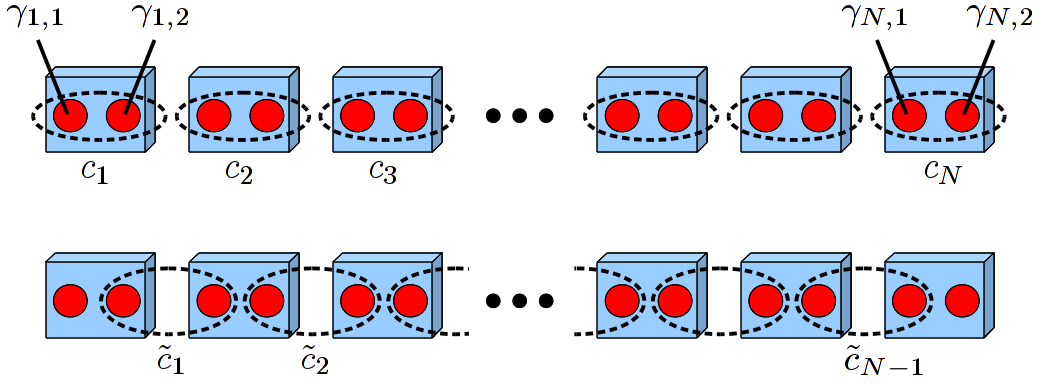
\includegraphics[width=\linewidth]{fig/ref/rys1.png}\\[1mm]
      {\footnotesize Góra: Majorany w~węzłach. Dół: parowanie między węzłami —
      $\gamma_{1,1}$ i~$\gamma_{N,2}$ zostają \alert{bez pary}.}
    \end{column}
  \end{columns}
  \zrodlo{Rys.: \LF{} rys.~1 (uwaga: w~podpisie oryginału indeksy końcowych Majoran są zamienione); równ.~(6)–(8)}
\end{frame}

% --- 11 (~1.5 min) -----------------------------------------------------------
\begin{frame}{Niesparowane Majorany i zdegenerowany stan podstawowy}
  \begin{itemize}
    \item $\gamma_{1,1}$ i~$\gamma_{N,2}$ \alert{nie występują} w~$H$. Razem tworzą jeden fermion:
          \[
            \tilde c_M = \tfrac12(\gamma_{N,2} + i\gamma_{1,1}),\qquad E_M = 0 .
          \]
    \item $\tilde c_M$ jest \alert{nielokalny}: połowa na lewym, połowa na prawym końcu.
    \item Stan podstawowy \alert{dwukrotnie zdegenerowany}:
          $\ket{0}$ i~$\ket{1} = \tilde c_M^\dagger\ket{0}$ —
          różnią się \alert{parzystością} liczby elektronów
          \[
            P = 1 - 2\tilde n_M = -i\,\gamma_{N,2}\gamma_{1,1}.
          \]
    \item Zwykły nadprzewodnik: niezdegenerowany stan podstawowy (parzysta liczba elektronów,
          kondensat par); tu dodanie elektronu kosztuje \alert{zero}.
    \item Żaden pomiar \alert{tylko na jednym końcu} nie rozróżni $\ket0$ od $\ket1$.
  \end{itemize}
  \zrodlo{\LF{} równ.~(9), rozdz.~2}
\end{frame}

% --- 12 (~1.5 min) -----------------------------------------------------------
\begin{frame}{Poza punktem specjalnym: faza topologiczna}
  \begin{columns}[T]
    \begin{column}{0.52\textwidth}
      Dla nieskończonego łańcucha (stała sieci $a=1$):
      \[
        E(k) = \pm\sqrt{(2t\cos k + \mu)^2 + 4\Delta^2\sin^2 k}
      \]
      \begin{itemize}
        \item Przerwa zamyka się tylko dla $|\mu| = 2t$ ($k=0$ lub $\pi$).
        \item $|\mu| < 2t$, $\Delta\neq 0$: \alert{faza topologiczna} —
              mody zerowe na końcach.
        \item $|\mu| > 2t$: faza trywialna, brak modów.
        \item Między fazami nie da się przejść \alert{bez zamknięcia przerwy}.
      \end{itemize}
    \end{column}
    \begin{column}{0.44\textwidth}
      \centering
      \begin{tikzpicture}[x=0.68cm, y=0.8cm]
        \fill[mBlue!15] (-2,0) rectangle (2,1.1);
        \draw[-{Stealth}] (-3.6,0) -- (3.8,0) node[right] {$\mu/t$};
        \foreach \x in {-2,2} \draw (\x,0.1) -- (\x,-0.1) node[below] {$\x$};
        \node[mBlue, font=\small, align=center] at (0,0.55) {topologiczna};
        \node[font=\scriptsize, gray] at (-2.9,0.55) {trywialna};
        \node[font=\scriptsize, gray] at (2.9,0.55) {trywialna};
        \fill[mRed] (-2,0) circle (2pt);
        \fill[mRed] (2,0) circle (2pt);
        \node[mRed, font=\scriptsize, align=center] at (0,-0.75) {zamknięcie przerwy\\ przy $|\mu|=2t$};
      \end{tikzpicture}
      \vspace{3mm}
      \begin{itemize}
        \item Mody końcowe nie są już punktowe: zanikają w~głąb
              jak $e^{-x/\xi}$.
        \item Odporność: małe zmiany $\mu$, $t$, $\Delta$ (także nieporządek)
              nie usuwają modów, dopóki przerwa jest otwarta.
      \end{itemize}
    \end{column}
  \end{columns}
  \zrodlo{\LF{} rozdz.~2; Kitaev (2001)}
\end{frame}

% --- 13 (~1.5 min) -----------------------------------------------------------
\begin{frame}{Symulacja: widmo BdG łańcucha $N = 30$}
  \begin{columns}[c]
    \begin{column}{0.49\textwidth}
      \centering
      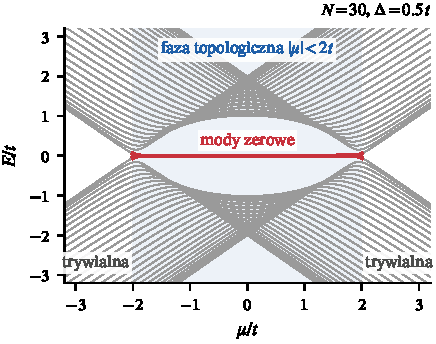
\includegraphics[width=\linewidth]{fig/kitaev_widmo.pdf}
    \end{column}
    \begin{column}{0.49\textwidth}
      \centering
      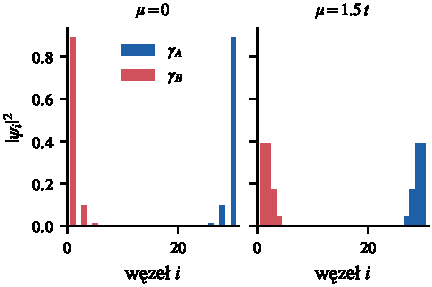
\includegraphics[width=\linewidth]{fig/kitaev_mody.pdf}
    \end{column}
  \end{columns}
  \vspace{1mm}
  {\small Diagonalizacja macierzy BdG $2N\times 2N$ (numpy), $\Delta = 0.5\,t$.
  Lewo: para stanów przy $E=0$ istnieje dokładnie dla $|\mu|<2t$.
  Prawo: dwie funkcje Majorany $\gamma_A$, $\gamma_B$ — zlokalizowane na
  \alert{przeciwnych końcach}; dla większego $\mu$ wnikają głębiej.}
  \zrodlo{Obliczenia własne: \texttt{sim/wykresy.py}}
\end{frame}

% --- 14 (~1 min) -------------------------------------------------------------
\begin{frame}{Rozszczepienie modów: $\delta E\propto e^{-L/\xi}$}
  \begin{columns}[c]
    \begin{column}{0.5\textwidth}
      \centering
      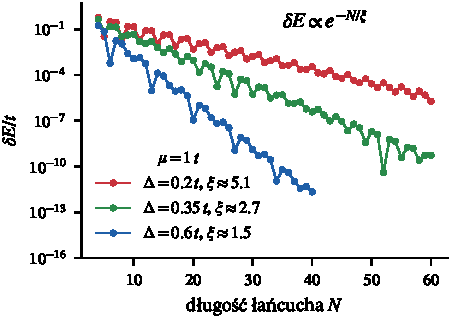
\includegraphics[width=\linewidth]{fig/kitaev_rozszczepienie.pdf}
    \end{column}
    \begin{column}{0.47\textwidth}
      \begin{itemize}
        \item W~skończonym łańcuchu ogony Majoran się nakładają →
              $\delta E \neq 0$, degeneracja tylko przybliżona.
        \item $\delta E \propto e^{-L/\xi}$ (z~oscylacjami), a~$\xi\sim\hbar v_F/\Delta$:
              mniejsza przerwa → \alert{dłuższy} mod.
        \item Wymóg konstrukcyjny: \alert{$L \gg \xi$}.
        \item W~nanodrucie $\xi$ to setki nm → drut rzędu $\unit{\micro\metre}$
              (cz.~II).
      \end{itemize}
    \end{column}
  \end{columns}
  \zrodlo{Obliczenia własne: \texttt{sim/wykresy.py}}
\end{frame}

% =============================================================================
\section{Parzystość, nieabelowość, kubit}
% =============================================================================

% --- 15 (~1.5 min) -----------------------------------------------------------
\begin{frame}{Kubit z czterech Majoran (tetron)}
  \begin{columns}[T]
    \begin{column}{0.5\textwidth}
      \begin{itemize}
        \item 2 Majorany = 1 fermion: $\ket0$, $\ket1$ mają różną parzystość →
              ich superpozycji nie da się utworzyć (reguła superselekcji). To \alert{nie} kubit.
        \item 4 Majorany, ustalona parzystość całkowita (np. parzysta):
              \[ \ket{\bar 0} = \ket{00},\qquad \ket{\bar 1} = \ket{11}. \]
        \item Operatory Pauliego = iloczyny par:
              \begin{align*}
                \sigma_z &= -i\gamma_1\gamma_2 = -i\gamma_3\gamma_4,\\
                \sigma_x &= -i\gamma_2\gamma_3,\qquad
                \sigma_y = -i\gamma_1\gamma_3.
              \end{align*}
      \end{itemize}
    \end{column}
    \begin{column}{0.46\textwidth}
      \centering
      \begin{tikzpicture}[scale=0.78]
        \fill[mBlue!25] (2.85,0.3) rectangle (3.15,1.6);
        \node[font=\tiny, rotate=90] at (3.45,0.95) {mostek SC};
        \shade[left color=gray!45, right color=gray!65, rounded corners=2pt] (0,1.6) rectangle (6,1.9);
        \shade[left color=gray!45, right color=gray!65, rounded corners=2pt] (0,0) rectangle (6,0.3);
        \foreach \p/\l/\a in {(0.2,1.75)/1/above, (5.8,1.75)/2/above, (5.8,0.15)/3/below, (0.2,0.15)/4/below}
          {\fill[mRed] \p circle (0.11); \node[\a=2pt, font=\small] at \p {$\gamma_\l$};}
        \draw[thick, mBlue, dashed] (0.2,2.25) .. controls (2,2.9) and (4,2.9) .. (5.8,2.25);
        \node[mBlue, font=\scriptsize] at (3,2.95) {$Z$: $-i\gamma_1\gamma_2$};
        \draw[thick, mGreen, dashed] (6.2,1.75) .. controls (6.9,1.4) and (6.9,0.5) .. (6.2,0.15);
        \node[mGreen, font=\scriptsize, align=left, anchor=west] at (6.75,0.95) {$X$:\\ $-i\gamma_2\gamma_3$};
      \end{tikzpicture}
      \vspace{2mm}
      {\footnotesize Odczyt kubitu = \alert{pomiar parzystości pary} Majoran.
      Wyspa nadprzewodząca z~energią ładowania $E_C$ chroni parzystość całkowitą.}
    \end{column}
  \end{columns}
  \zrodlo{\LF{} równ.~(28)–(30); Karzig i in., PRB 95, 235305 (2017)}
\end{frame}

% --- 16 (~1.5 min) -----------------------------------------------------------
\begin{frame}{Wymiana (braiding) i statystyka nieabelowa}
  \begin{columns}[T]
    \begin{column}{0.5\textwidth}
      Wymiana $\gamma_i \leftrightarrow \gamma_j$:
      \[
        U_{ij} = e^{\frac{\pi}{4}\gamma_i\gamma_j} = \tfrac{1}{\sqrt2}\bigl(1 + \gamma_i\gamma_j\bigr),
      \]
      \[
        \gamma_i \to -\gamma_j,\qquad \gamma_j \to \gamma_i .
      \]
      Na stanach:
      \begin{align*}
        U_{12}\ket{00} &= e^{i\pi/4}\ket{00} &&\text{(tylko faza)}\\
        U_{23}\ket{00} &= \tfrac{1}{\sqrt2}\bigl(\ket{00} + i\ket{11}\bigr) &&\text{(superpozycja!)}
      \end{align*}
    \end{column}
    \begin{column}{0.46\textwidth}
      \begin{block}{Nieabelowość}
        \[ [U_{i-1,i},\,U_{i,i+1}] = \gamma_{i-1}\gamma_{i+1} \neq 0 \]
        Kolejność wymian ma znaczenie.
      \end{block}
      \begin{itemize}
        \item W~bazie kubitu: $U_{12} = e^{i\pi\sigma_z/4}$,
              $U_{23} = e^{i\pi\sigma_x/4}$ — obroty o~$\pi/2$.
        \item Wynik zależy tylko od \alert{topologii} ścieżek (warkocza), nie od
              czasu czy kształtu.
        \item Wymiana wymaga 2D — w~drutach: złącza T.
      \end{itemize}
    \end{column}
  \end{columns}
  \zrodlo{\LF{} równ.~(19)–(27), (31)–(32) (znak wykładnika w~(31)–(32) poprawiony zgodnie z~(22)–(25)); D.\,A.~Ivanov, PRL 86, 268 (2001); Alicea i in., Nat.~Phys. 7, 412 (2011)}
\end{frame}

% --- 17 (~1 min) -------------------------------------------------------------
\begin{frame}{Co jest chronione, a co nie}
  \begin{columns}[T]
    \begin{column}{0.47\textwidth}
      \begin{block}{Chronione}
        \begin{itemize}
          \item Zaburzenia lokalne: zmiana stanu wymaga operatora $\gamma_i\gamma_j$
                — dla odległych Majoran tłumionego $\propto e^{-L/\xi}$.
          \item Fazy bramek z~wymian są dokładne (topologiczne).
        \end{itemize}
      \end{block}
    \end{column}
    \begin{column}{0.49\textwidth}
      \begin{alertblock}{Niechronione}
        \begin{itemize}
          \item \alert{Zatruwanie kwazicząstkami}: elektron z~zewnątrz
                ($\propto\gamma_i$) zmienia parzystość — odległość nie pomaga.
          \item Skończone $\delta E\propto e^{-L/\xi}$ → powolny obrót fazy.
          \item Wzbudzenia termiczne $\propto e^{-\Delta_\mathrm{top}/k_BT}$.
          \item Wymiany dają tylko \alert{bramki Clifforda} → brak uniwersalności;
                bramka $T$ ($\pi/8$) wymaga niechronionych metod (stany magiczne).
        \end{itemize}
      \end{alertblock}
    \end{column}
  \end{columns}
  \zrodlo{\LF{} rozdz.~3.3; Nayak i in., Rev.~Mod.~Phys. 80, 1083 (2008)}
\end{frame}

% --- 18 (~1 min) -------------------------------------------------------------
\begin{frame}{Obliczenia oparte na pomiarach}
  \begin{columns}[c]
    \begin{column}{0.5\textwidth}
      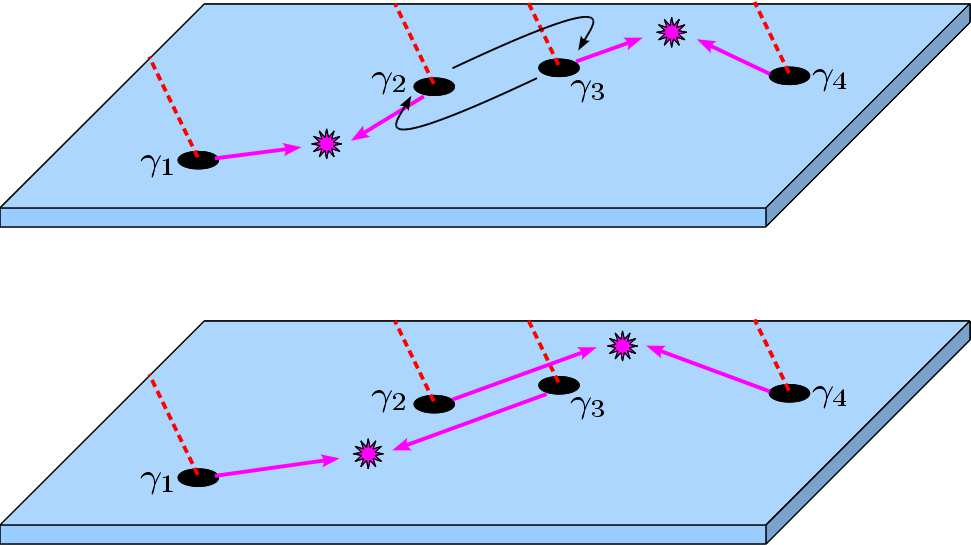
\includegraphics[width=\linewidth]{fig/ref/rys3.png}
    \end{column}
    \begin{column}{0.47\textwidth}
      \begin{itemize}
        \item Fizyczne przesuwanie Majoran jest trudne.
        \item Górny panel: wymiana $2\leftrightarrow3$, potem pomiar par $(1,2)$, $(3,4)$.\\
              Dolny panel: \alert{bez wymiany} — pomiar par $(1,3)$, $(2,4)$.
              Statystyka wyników taka sama.
        \item Wymianę można zastąpić \alert{sekwencją pomiarów parzystości}
              (measurement-only TQC).
        \item Dlatego kluczowym eksperymentem jest \alert{szybki, wierny pomiar
              parzystości} pary Majoran (→ cz.~II).
      \end{itemize}
    \end{column}
  \end{columns}
  \zrodlo{Rys.: \LF{} rys.~3; Bonderson, Freedman, Nayak, PRL 101, 010501 (2008)}
\end{frame}

% =============================================================================
\section{Nanodrut półprzewodnikowy — model}
% =============================================================================

% --- 19 (~1 min) -------------------------------------------------------------
\begin{frame}{Realizacja: nanodrut + nadprzewodnik + pole $B$}
  \begin{columns}[c]
    \begin{column}{0.5\textwidth}
      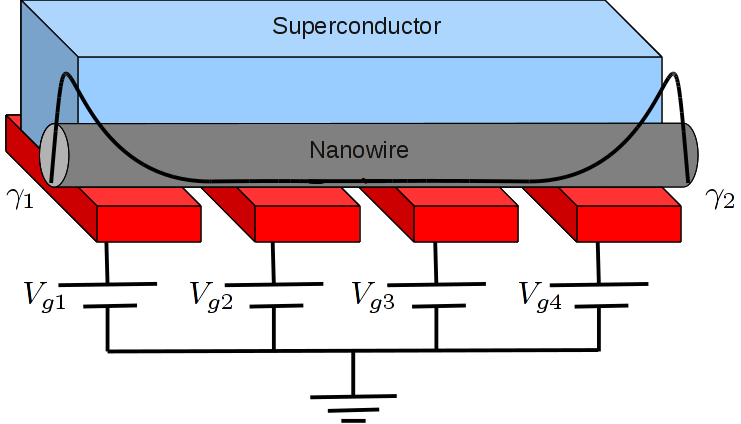
\includegraphics[width=\linewidth]{fig/ref/rys4.png}
    \end{column}
    \begin{column}{0.47\textwidth}
      \begin{itemize}
        \item Drut InAs lub InSb: silne SOC, duże $|g|$, mała $m^*$;
              średnica $\sim\qty{100}{\nano\metre}$ \sprawdz.
        \item Powłoka nadprzewodząca (Al, NbTiN) → indukowana przerwa $\Delta$.
        \item Pole $B$ \alert{wzdłuż drutu}, tj.\ prostopadle do pola spin–orbita.
        \item Bramki $V_{g1\ldots g4}$: lokalny $\mu$, bariery tunelowe, kropki.
        \item W~fazie topologicznej: $\gamma_1$, $\gamma_2$ na końcach,
              zanik wykładniczy w~głąb drutu.
      \end{itemize}
    \end{column}
  \end{columns}
  \zrodlo{Rys.: \LF{} rys.~4; Lutchyn i in., PRL 105, 077001 (2010); Oreg i in., PRL 105, 177002 (2010)}
\end{frame}

% --- 20 (~1.5 min) -----------------------------------------------------------
\begin{frame}{Pasma drutu ze sprzężeniem spin–orbita i polem Zeemana}
  \[
    H_0 = \frac{\hbar^2k^2}{2m^*} - \mu + \alpha k\,\sigma_y + V_Z\,\sigma_z,
    \qquad
    E_\pm(k) = \frac{\hbar^2k^2}{2m^*} - \mu \pm \sqrt{\alpha^2k^2 + V_Z^2},
    \qquad V_Z = \tfrac12 g\mu_B B
  \]
  \centering
  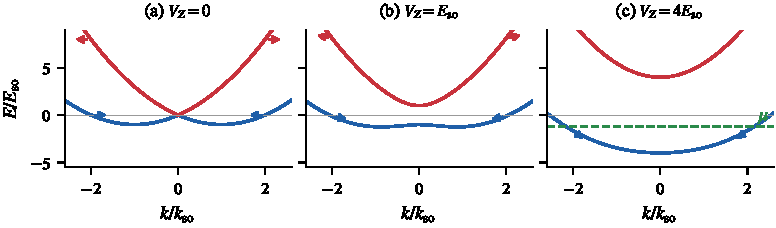
\includegraphics[width=0.8\linewidth]{fig/drut_pasma.pdf}\\[-1mm]
  \raggedright\small
  (a) SOC przesuwa parabole o~$\pm k_\mathrm{so}$, spin $\parallel\pm y$.
  (b) $V_Z$ otwiera przerwę $2V_Z$ przy $k=0$.
  (c) $\mu$ w~przerwie → tylko \alert{jedna} para punktów Fermiego — „bezspinowo”, ale spiny
  przy $\pm k_F$ nie są równoległe, więc s-wave wciąż może parować.
  {\footnotesize ($k_\mathrm{so}=m^*\alpha/\hbar^2$, \ $E_\mathrm{so}=m^*\alpha^2/2\hbar^2$)}
  % UWAGA dla prelegenta: w [LF12] równ. (51)–(53) czynnik 1/2 przy członie Zeemana jest
  % niekonsekwentny (w (51) jest B̃σ_z/2, w (52)–(53) już B̃). Tu V_Z = współczynnik przy σ_z.
  \zrodlo{Odtworzenie \LF{} rys.~5a–c (obliczenia własne)}
\end{frame}

% --- 21 (~1.5 min) -----------------------------------------------------------
\begin{frame}{Dodajemy nadprzewodnictwo: hamiltonian BdG}
  \[
    H_\mathrm{BdG}(k) = \Bigl(\frac{\hbar^2k^2}{2m^*} - \mu + \alpha k\,\sigma_y\Bigr)\tau_z
                        + V_Z\,\sigma_z + \Delta\,\tau_x ,
    \qquad
    E(k{=}0) = \pm V_Z \pm \sqrt{\Delta^2 + \mu^2}
  \]
  \centering
  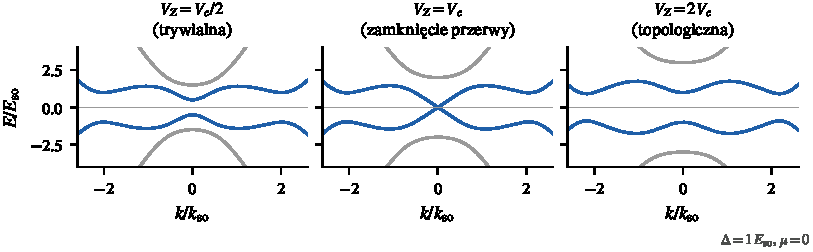
\includegraphics[width=0.9\linewidth]{fig/drut_bdg.pdf}\\
  \raggedright\small
  Przy $k=0$ przerwa $\abs{V_Z - \sqrt{\Delta^2+\mu^2}}$ \alert{zamyka się} dla
  $V_Z = V_c \equiv \sqrt{\Delta^2+\mu^2}$ i~otwiera ponownie — już w~fazie topologicznej.
  Przerwa przy $k_F$ jest $\propto\Delta$, ale maleje z~$B$ (cz.~II).
  \zrodlo{Odtworzenie \LF{} rys.~5d dla trzech wartości $V_Z$ (obliczenia własne); \LF{} równ.~(37)–(40)}
\end{frame}

% --- 22 (~1.5 min) -----------------------------------------------------------
\begin{frame}{Warunek topologiczny: $V_Z > \sqrt{\Delta^2+\mu^2}$}
  \begin{columns}[c]
    \begin{column}{0.55\textwidth}
      \centering
      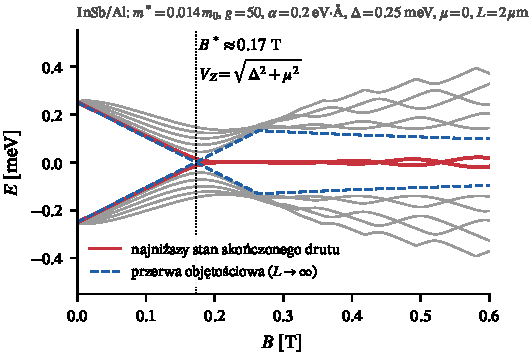
\includegraphics[width=\linewidth]{fig/drut_EB.pdf}
    \end{column}
    \begin{column}{0.43\textwidth}
      \[
        B > B^* = \frac{2\sqrt{\Delta^2+\mu^2}}{g\,\mu_B}
      \]
      \begin{itemize}
        \item Drut $L=\qty{2}{\micro\metre}$, ciasne wiązanie, $a=\qty{10}{\nano\metre}$.
        \item $B<B^*$: przerwa maleje, brak stanów przy $E=0$.
        \item $B=B^*$: \alert{zamknięcie przerwy}.
        \item $B>B^*$: mod zerowy; \alert{oscylacje} $\delta E$ rosną z~$B$ (rośnie $\xi$).
      \end{itemize}
      \vspace{1mm}
      {\small Sygnatura: zamknięcie i~ponowne otwarcie przerwy \alert{+} mod zerowy.}
    \end{column}
  \end{columns}
  \zrodlo{Obliczenia własne (\texttt{sim/wykresy.py}); \LF{} równ.~(53)}
\end{frame}

% =============================================================================
%  CZĘŚĆ II — Prelegent B (slajdy 23–42, ~27 min)
% =============================================================================
\renewcommand{\prelegent}{cz.\,II — Prelegent B}

% =============================================================================
\section{Nanodrut — inżynieria}
% =============================================================================

% --- 23 (~1.5 min) -----------------------------------------------------------
\begin{frame}{Efektywna przerwa p-wave i kompromisy}
  \begin{columns}[T]
    \begin{column}{0.5\textwidth}
      Granica $V_Z\gg E_\mathrm{so},\Delta$, $\mu\approx0$: rzut na dolne pasmo
      (spin $\approx\,\downarrow$ + domieszka $\propto\alpha k/V_Z$):
      \small
      \[
        H_\mathrm{eff} \simeq \!\int\! dx\Bigl[\Psi_-^\dagger\Bigl(\tfrac{\hbar^2k^2}{2m^*} - V_Z\Bigr)\Psi_-
        + \Delta_p\,\Psi_-\,k\,\Psi_- + \hc\Bigr]
      \]
      \[
        \Delta_p \approx \frac{\alpha}{V_Z}\,\Delta,\qquad
        \Delta_\mathrm{eff} = \Delta_p k_F \approx \frac{\alpha k_F}{V_Z}\,\Delta
      \]
      To jest model p-wave (równ.~(10) w~\LF) → łańcuch Kitaeva.
    \end{column}
    \begin{column}{0.46\textwidth}
      \begin{block}{Kompromisy}
        \begin{itemize}
          \item $B\uparrow$: szersze okno $|\mu| < \sqrt{V_Z^2-\Delta^2}$, ale
                $\Delta_\mathrm{eff}\downarrow$, $\xi\uparrow$, nadprzewodnik słabnie.
          \item $\alpha\uparrow$: większe $\Delta_\mathrm{eff}$, krótsze $\xi$ — ale
                $\alpha$ zależy od pola bramek, trudno je kontrolować.
          \item $|g|\uparrow$: to samo $V_Z$ przy mniejszym $B$ (mniej szkody dla Al).
          \item Nie przesadzać z~$V_Z/E_\mathrm{so}$ — rośnie wrażliwość na nieporządek.
        \end{itemize}
      \end{block}
    \end{column}
  \end{columns}
  \zrodlo{\LF{} równ.~(54) i~rozdz.~5; J.~Alicea, Rep.~Prog.~Phys. 75, 076501 (2012)}
\end{frame}

% --- 24 (~1.5 min) -----------------------------------------------------------
\begin{frame}{Skale energii — liczby}
  \begin{columns}[T]
    \begin{column}{0.55\textwidth}
      \centering
      \begin{tabular}{@{}lcc@{}}
        \toprule
        & InSb & InAs \\
        \midrule
        $m^*/m_0$ & 0.014 & 0.023 \\
        $|g|$ (drut) & 40–50 & 10–15 \\
        $\tfrac12|g|\mu_B$ [\unit{\milli\electronvolt\per\tesla}] & 1.2–1.45 & 0.29–0.43 \\
        $B^*$ ($\Delta=\qty{0.2}{\milli\electronvolt}$, $\mu=0$) & \alert{0.14–0.17\,T} & \alert{0.46–0.69\,T} \\
        \bottomrule
      \end{tabular}\\[2mm]
      {\footnotesize $\mu_B = \qty{57.9}{\micro\electronvolt\per\tesla}$; wartości
      orientacyjne \sprawdz[zweryfikować z~literaturą]}
    \end{column}
    \begin{column}{0.42\textwidth}
      \begin{itemize}
        \item $\Delta_\mathrm{Al} \approx \qty{0.2}{\milli\electronvolt}$
        \item $k_B\cdot\qty{20}{\milli\kelvin} \approx \qty{1.7}{\micro\electronvolt}$
              $\ll \Delta$ — ale $\Delta_\mathrm{top}$ bywa rzędu
              \qty{10}{\micro\electronvolt}–\qty{50}{\micro\electronvolt} \sprawdz
        \item InSb, $\alpha = \qty{0.2}{\electronvolt\angstrom}$:
              $l_\mathrm{so} = \hbar^2/m^*\alpha \approx \qty{270}{\nano\metre}$,
              $E_\mathrm{so}\approx\qty{37}{\micro\electronvolt}$
        \item Nasz model: $\xi\approx\qty{0.3}{\micro\metre}$–\qty{0.8}{\micro\metre}
              dla $B=\qty{0.25}{\tesla}$–\qty{0.5}{\tesla}
              → drut \alert{\qty{1}{\micro\metre}–\qty{3}{\micro\metre}}
      \end{itemize}
    \end{column}
  \end{columns}
\end{frame}

% --- 25 (~1.5 min) -----------------------------------------------------------
\begin{frame}{Komplikacje w realnym drucie}
  \begin{itemize}
    \item \alert{Wiele podpasm}: w~drucie $\sim\qty{100}{\nano\metre}$ obsadzonych jest kilka
          podpasm; faza topologiczna wymaga nieparzystej liczby, okna $\mu$ się zawężają.
    \item \alert{Efekty orbitalne} pola: strumień przez przekrój
          ($\Phi_0 = h/e$ dla $d=\qty{100}{\nano\metre}$ przy $B\approx\qty{0.5}{\tesla}$)
          zmniejsza przerwę i~zmienia efektywne $g$.
    \item \alert{„Metalizacja”}: silne sprzężenie z~Al daje dużą przerwę indukowaną,
          ale renormalizuje $g^*$, $\alpha$ w~dół i~przesuwa $\mu$ (zagięcie pasm na
          granicy) — kompromis słabe/silne sprzężenie.
    \item \alert{Nieporządek}: fluktuacje $\mu$ wzdłuż drutu (defekty, ładunki
          w~tlenku, chropowatość) $\gtrsim\Delta_\mathrm{eff}$ → fragmentacja fazy,
          trywialne stany przy $E\approx0$.
    \item \alert{Elektrostatyka bramek}: $\mu$ i~$\alpha$ zależą od pola bramek,
          ekranowanego przez Al → potrzebne symulacje Schrödinger–Poisson.
  \end{itemize}
  \zrodlo{Lutchyn i in., Nat.~Rev.~Mater. 3, 52 (2018); Prada i in., Nat.~Rev.~Phys. 2, 575 (2020)}
\end{frame}

% =============================================================================
\section{Materiały i technologia}
% =============================================================================

% --- 26 (~1.5 min) -----------------------------------------------------------
\begin{frame}{Materiały}
  \small
  \textbf{Półprzewodniki} \sprawdz[wartości orientacyjne]\\[1mm]
  \begin{tabularx}{\linewidth}{@{}lcccX@{}}
    \toprule
    & $E_g$ (\qty{0}{\kelvin}) [\unit{\electronvolt}] & $m^*/m_0$ & $|g|$ & uwagi \\
    \midrule
    InAs & 0.42 & 0.023 & $\sim15$ & warstwa akumulacyjna na powierzchni → dobry kontakt z~Al, bez bariery Schottky'ego \\
    InSb & 0.24 & 0.014 & $\sim50$ & największe $|g|$ i~SOC; trudniejszy wzrost \\
    PbTe & 0.19 & anizotr. & duże & $\varepsilon_r\sim10^3$ ekranuje nieporządek ładunkowy \\
    \bottomrule
  \end{tabularx}\\[3mm]
  \textbf{Nadprzewodniki}\\[1mm]
  \begin{tabularx}{\linewidth}{@{}lcccX@{}}
    \toprule
    & $T_c$ [\unit{\kelvin}] & $\Delta$ [\unit{\milli\electronvolt}] & $B_c$ (lity) & uwagi \\
    \midrule
    Al    & 1.2   & 0.18–0.25 & \qty{10}{\milli\tesla} & epitaksja na InAs/InSb; cienka warstwa: $B_{c\parallel}\sim\qty{2}{\tesla}$ \sprawdz \\
    NbTiN & 13–15 & $\sim$2   & $>\qty{10}{\tesla}$    & napylany (Delft 2012), miękka przerwa \\
    Pb    & 7.2   & 1.35      & \qty{80}{\milli\tesla} & duża przerwa; epitaksja na InAs, PbTe \\
    Sn    & 3.7   & 0.57      & \qty{30}{\milli\tesla} & $\beta$-Sn na InSb, odporny na pole w~cienkiej powłoce \\
    \bottomrule
  \end{tabularx}
  \zrodlo{Kanne i in., Nat.~Nanotechnol. 16, 776 (2021) (Pb); Pendharkar i in., Science 372, 508 (2021) (Sn)}
\end{frame}

% --- 27 (~1.5 min) -----------------------------------------------------------
\begin{frame}{Wzrost: VLS i epitaksjalna powłoka in situ}
  \begin{columns}[T]
    \begin{column}{0.5\textwidth}
      \begin{block}{VLS (vapor–liquid–solid)}
        \begin{itemize}
          \item Katalizator: kropla Au; MBE lub MOVPE.
          \item Wzrost wzdłuż [111]B / [0001]; średnica ≈ średnica kropli.
          \item InSb często na „łodydze” InP/InAs.
        \end{itemize}
      \end{block}
      \begin{block}{Epitaksjalny Al in situ}
        \begin{itemize}
          \item Bez przerywania próżni, po schłodzeniu podłoża; kilka–kilkanaście nm
                na 1–3 ściankach → ostra, czysta granica faz.
        \end{itemize}
      \end{block}
    \end{column}
    \begin{column}{0.46\textwidth}
      \begin{block}{Cieniowanie (shadowing)}
        \begin{itemize}
          \item Sąsiednie druty / struktury zasłaniają kierunkową wiązkę Al
                → przerwy w~powłoce \alert{bez trawienia}.
          \item Trawienie Al na mokro może uszkodzić powierzchnię półprzewodnika.
        \end{itemize}
      \end{block}
      \vspace{2mm}
      \sprawdz[dodać zdjęcie SEM/TEM z~Krogstrup 2015 lub Gazibegovic 2017, z~podaniem źródła]
    \end{column}
  \end{columns}
  \zrodlo{Krogstrup i in., Nat.~Mater. 14, 400 (2015); Gazibegovic i in., Nature 548, 434 (2017)}
\end{frame}

% --- 28 (~1.5 min) -----------------------------------------------------------
\begin{frame}{Twarda vs miękka przerwa}
  \begin{columns}[c]
    \begin{column}{0.46\textwidth}
      \centering
      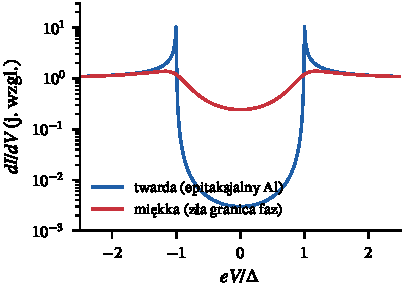
\includegraphics[width=\linewidth]{fig/przerwa_twarda_miekka.pdf}\\
      {\scriptsize Schemat: gęstość stanów Dynesa,
      $\Gamma = 0.003\Delta$ vs $0.25\Delta$}
    \end{column}
    \begin{column}{0.5\textwidth}
      \begin{itemize}
        \item \alert{Miękka przerwa}: stany w~przerwie od nieporządku na granicy faz
              (Al/NbTiN napylany ex situ po usunięciu tlenku).
        \item Skutki: kwazicząstki w~przerwie → zatruwanie, fałszywe piki, brak ochrony.
        \item \alert{Twarda przerwa} (epitaksjalne InAs/Al): przewodnictwo w~przerwie
              stłumione do $\sim100\times$ względem stanu normalnego.
        \item Warunek konieczny dla wszystkich dalszych eksperymentów.
      \end{itemize}
    \end{column}
  \end{columns}
  \zrodlo{Chang i in., Nat.~Nanotechnol. 10, 232 (2015); Krogstrup i in., Nat.~Mater. 14, 400 (2015)}
\end{frame}

% --- 29 (~1.5 min) -----------------------------------------------------------
\begin{frame}{Skalowalne platformy: SAG i 2DEG InAs/Al}
  \begin{columns}[T]
    \begin{column}{0.48\textwidth}
      \begin{block}{SAG — selective-area growth}
        \begin{itemize}
          \item Wzrost tylko w~oknach maski (SiO$_2$) na podłożu
                → druty \alert{w~płaszczyźnie}, dowolne sieci (złącza T, pętle).
          \item Litografia zamiast przenoszenia pojedynczych drutów.
        \end{itemize}
      \end{block}
    \end{column}
    \begin{column}{0.48\textwidth}
      \begin{block}{2DEG InAs/Al (Microsoft)}
        \begin{itemize}
          \item Płytka studnia kwantowa InAs + epitaksjalny Al na całej płytce.
          \item Drut definiowany litografią: wytrawienie Al + bramki zubożające.
          \item Ta platforma stoi za TGP (2023), odczytem parzystości (2025) i~tetronem.
        \end{itemize}
      \end{block}
    \end{column}
  \end{columns}
  \vspace{2mm}
  \begin{itemize}
    \item Plusy: technologia planarna, skalowanie, integracja z~odczytem.
          Minusy: nieporządek w~studni, mniejsze $|g|$ → potrzebne pola $\sim\qty{2}{\tesla}$.
  \end{itemize}
  \zrodlo{Vaitiekėnas i in., PRL 121, 147701 (2018); Shabani i in., PRB 93, 155402 (2016); Microsoft Quantum, PRB 107, 245423 (2023)}
\end{frame}

% --- 30 (~1 min) -------------------------------------------------------------
\begin{frame}{Układ pomiarowy}
  \begin{columns}[T]
    \begin{column}{0.5\textwidth}
      \begin{itemize}
        \item \alert{Bramki}: Ti/Au pod lub nad drutem, dielektryk HfO$_2$ (ALD);
              ustalają $\mu$, bariery tunelowe, kropki kwantowe.
        \item \alert{Kontakty} normalne po usunięciu tlenku (trawienie jonowe, pasywacja siarką).
        \item \alert{Kriostat rozcieńczalnikowy}: $T\approx\qty{10}{\milli\kelvin}$–\qty{20}{\milli\kelvin}
              (temperatura elektronów zwykle wyższa — filtrowanie linii).
      \end{itemize}
    \end{column}
    \begin{column}{0.46\textwidth}
      \begin{itemize}
        \item \alert{Magnes wektorowy}: precyzyjne ustawienie $B\parallel$ drut
              ($\perp$ pola spin–orbita).
        \item \alert{Lock-in}: małe wzbudzenie AC na napięciu DC → $dI/dV(V)$.
        \item \alert{Reflektometria RF}: obwód rezonansowy LC, odczyt ładunku/pojemności
              w~skali \unit{\micro\second} — podstawa pomiaru parzystości.
      \end{itemize}
    \end{column}
  \end{columns}
  \vspace{2mm}
  \centering
  $k_BT \approx \qty{1.7}{\micro\electronvolt}\ \ll\ \Delta_\mathrm{top}\ \lesssim\ \Delta\approx\qty{200}{\micro\electronvolt}$
\end{frame}

% =============================================================================
\section{Pomiary i pułapki}
% =============================================================================

% --- 31 (~1.5 min) -----------------------------------------------------------
\begin{frame}{Spektroskopia tunelowa i pik przy zerowym napięciu}
  \begin{columns}[T]
    \begin{column}{0.5\textwidth}
      \begin{itemize}
        \item Układ N–bariera–drut: $dI/dV(V)\propto$ lokalna gęstość stanów
              na końcu drutu (słabe tunelowanie, $T\to0$).
        \item Majorana → \alert{pik przy zerowym napięciu} (ZBP),
              stabilny w~szerokim zakresie $B$ i~$V_g$.
        \item Rezonansowe odbicie Andreeva przez mod Majorany:
              \[ G(V{=}0) = \frac{2e^2}{h}\quad (T=0), \]
              niezależnie od przezroczystości bariery.
      \end{itemize}
    \end{column}
    \begin{column}{0.46\textwidth}
      \begin{block}{Czego oczekujemy od prawdziwej Majorany}
        \begin{itemize}
          \item ZBP pojawia się dla $B>B^*$, razem z~zamknięciem i~otwarciem przerwy.
          \item Pik na \alert{obu końcach} jednocześnie.
          \item Wysokość $\to 2e^2/h$ przy $k_BT\ll\Gamma$.
          \item Znika, gdy $B$ obrócone $\parallel$ pola SO.
        \end{itemize}
      \end{block}
    \end{column}
  \end{columns}
  \zrodlo{Law, Lee, Ng, PRL 103, 237001 (2009); K.~Flensberg, PRB 82, 180516 (2010)}
\end{frame}

% --- 32 (~1.5 min) -----------------------------------------------------------
\begin{frame}{Delft 2012 — Mourik i in.}
  \begin{columns}[T]
    \begin{column}{0.5\textwidth}
      \begin{itemize}
        \item Nanodrut InSb + NbTiN, kontakt Au, bramki lokalne.
        \item ZBP pojawia się przy $B\sim\qty{0.1}{\tesla}$ i~trwa do
              $\sim\qty{1}{\tesla}$ \sprawdz.
        \item Testy kontrolne: brak piku bez nadprzewodnika i~dla $B$ ustawionego
              wzdłuż pola SO.
      \end{itemize}
      \sprawdz[dodać wykres $dI/dV(B,V)$ z~pracy, z~podaniem źródła]
    \end{column}
    \begin{column}{0.46\textwidth}
      \begin{alertblock}{Problemy}
        \begin{itemize}
          \item Wysokość piku $\sim0.05\cdot2e^2/h$ zamiast $2e^2/h$ \sprawdz.
          \item Miękka przerwa (NbTiN napylany).
          \item Nie widać zamknięcia przerwy objętościowej.
        \end{itemize}
      \end{alertblock}
      \vspace{1mm}
      Podobne wyniki w~2012: Deng i in.\ (InSb–Nb), Das i in.\ (InAs–Al).
    \end{column}
  \end{columns}
  \zrodlo{V.~Mourik i in., Science 336, 1003 (2012)}
\end{frame}

% --- 33 (~1.5 min) -----------------------------------------------------------
\begin{frame}{Kwantyzacja $2e^2/h$ i retrakcja}
  \begin{itemize}
    \item Zhang i in., Nature 556, 74 (2018): plateau $G\approx2e^2/h$ ZBP w~InSb/Al
          (epitaksjalny) — przedstawione jako silny dowód Majoran.
    \item Analiza pełnych danych (2020–21): selektywny dobór zakresów,
          korekta oporu szeregowego zmieniała wniosek; pełny zestaw nie wspierał tezy.
          \alert{Retrakcja w~2021.}
  \end{itemize}
  \vspace{2mm}
  \begin{block}{Lekcje}
    \begin{enumerate}
      \item Plateau bliskie $2e^2/h$ mogą dawać też \alert{trywialne} stany.
      \item Pełne dane i~kod analizy, z~góry ustalone kryteria.
      \item Pojedyncza \alert{lokalna} sygnatura (jeden koniec, jeden pik) nie wystarcza.
    \end{enumerate}
  \end{block}
  \zrodlo{H.~Zhang i in., Nature 556, 74 (2018), wycofana 2021 \sprawdz[dodać odnośnik do noty o~retrakcji]}
\end{frame}

% --- 34 (~1.5 min) -----------------------------------------------------------
\begin{frame}{Podróbki: co jeszcze daje pik przy zerze}
  \begin{columns}[T]
    \begin{column}{0.5\textwidth}
      \begin{itemize}
        \item \alert{Trywialne stany Andreeva (ABS)}: w~kropce na końcu drutu
              lub przy gładkim potencjale mogą „przykleić się” do $E=0$ w~szerokim zakresie $B$.
        \item \alert{Quasi-Majorany}: dwie Majorany \emph{tego samego} końca,
              częściowo rozdzielone — lokalnie nie do odróżnienia.
      \end{itemize}
    \end{column}
    \begin{column}{0.46\textwidth}
      \begin{itemize}
        \item \alert{Efekt Kondo}: spin w~kropce daje ZBP (rozszczepia się w~polu).
        \item \alert{Nieporządek}: antylokalizacja w~klasie D → szeroki ZBP
              bez Majoran.
      \end{itemize}
    \end{column}
  \end{columns}
  \vspace{3mm}
  \begin{alertblock}{Wniosek}
    Spektroskopia tunelowa jednego końca \alert{nie rozstrzyga}.
    Potrzebne pomiary nielokalne i~sprawdzenie parzystości.
  \end{alertblock}
  \zrodlo{Liu, Sau, Das Sarma, PRB 96, 075161 (2017); Vuik i in., SciPost Phys. 7, 061 (2019); Lee i in., PRL 109, 186802 (2012); Pikulin i in., NJP 14, 125011 (2012) \sprawdz[sprawdzić numery]}
\end{frame}

% --- 35 (~1.5 min) -----------------------------------------------------------
\begin{frame}{Lepsze testy}
  \begin{columns}[T]
    \begin{column}{0.49\textwidth}
      \begin{itemize}
        \item \alert{Przewodnictwo nielokalne} (3 końcówki):
              $G_{LR} = dI_L/dV_R$ mierzy przerwę \emph{objętościową} →
              widać zamknięcie i~ponowne otwarcie.
        \item \alert{TGP} (topological gap protocol): ZBP na obu końcach +
              zamknięcie/otwarcie przerwy nielokalnej w~obszarze $(B,V_g)$,
              kryteria statystyczne. Microsoft, PRB 2023.
      \end{itemize}
    \end{column}
    \begin{column}{0.47\textwidth}
      \begin{itemize}
        \item \alert{Wyspy Coulombowskie}: okres pików $2e\to1e$ dla $B>B^*$;
              rozszczepienie maleje wykładniczo z~długością wyspy
              (Albrecht i in.\ 2016).
        \item \alert{Efekt Josephsona $4\pi$}: prąd okresowy w~fazie z~okresem $4\pi$
              → brak nieparzystych stopni Shapiro. Kłopot: zatruwanie,
              przejścia Landaua–Zenera.
      \end{itemize}
    \end{column}
  \end{columns}
  \zrodlo{Rosdahl i in., PRB 97, 045421 (2018); Microsoft Quantum, PRB 107, 245423 (2023); Albrecht i in., Nature 531, 206 (2016); Rokhinson i in., Nat.~Phys. 8, 795 (2012); Laroche i in., Nat.~Commun. 10, 245 (2019)}
\end{frame}

% --- 36 (~2 min) -------------------------------------------------------------
\begin{frame}{Odczyt parzystości przez pojemność kwantową}
  \begin{columns}[c]
    \begin{column}{0.44\textwidth}
      \centering
      \begin{tikzpicture}[scale=0.8]
        \fill[mBlue!25] (0,0.3) rectangle (5,0.45);
        \shade[left color=gray!45, right color=gray!65, rounded corners=2pt] (0,0) rectangle (5,0.3);
        \fill[mRed] (0.2,0.15) circle (0.1) node[below=3pt, black, font=\small] {$\gamma_1$};
        \fill[mRed] (4.8,0.15) circle (0.1) node[below=3pt, black, font=\small] {$\gamma_2$};
        \draw[fill=mGreen!30, draw=mGreen] (0.2,1.5) circle (0.3) node {\scriptsize QD};
        \draw[thick, mGreen] (0.2,1.2) -- (0.2,0.5);
        \draw[thick, mGreen] (0.5,1.5) -- (4.8,1.5) -- (4.8,0.5);
        \node[font=\small] at (2.5,1.0) {$\Phi$};
        \draw[-{Stealth}] (-0.2,1.5) -- (-1.1,1.5) node[left, font=\scriptsize, align=center] {rezonator\\ RF};
      \end{tikzpicture}\\[1mm]
      {\scriptsize Schemat: kropka sprzężona z~oboma końcami drutu tworzy interferometr ze strumieniem $\Phi$.}
    \end{column}
    \begin{column}{0.53\textwidth}
      \begin{itemize}
        \item Energia układu kropka–drut zależy od parzystości $i\gamma_1\gamma_2$ i~$\Phi$
              → \alert{pojemność kwantowa} $C_Q\propto\partial^2E/\partial n_g^2$ też.
        \item Odczyt: przesunięcie częstotliwości rezonatora (reflektometria RF).
        \item Microsoft, Nature 2025 (InAs/Al 2DEG, $B\approx\qty{2}{\tesla}$):
              pomiar \alert{jednostrzałowy}, błąd przypisania $\approx1\%$,
              czas przełączania parzystości $\gtrsim\qty{1}{\milli\second}$ \sprawdz.
        \item Nota redakcji: pomiar \alert{nie rozstrzyga}, czy stany są topologiczne.
      \end{itemize}
    \end{column}
  \end{columns}
  \zrodlo{Microsoft Azure Quantum, Nature 638, 651 (2025)}
\end{frame}

% =============================================================================
\section{Stan na 2026}
% =============================================================================

% --- 37 (~1.5 min) -----------------------------------------------------------
\begin{frame}{Łańcuchy Kitaeva z kropek kwantowych}
  \begin{columns}[T]
    \begin{column}{0.52\textwidth}
      \begin{itemize}
        \item Kropki kwantowe = węzły łańcucha Kitaeva.
              $t$: zwykłe tunelowanie (ECT), $\Delta$: krzyżowe odbicie Andreeva (CAR)
              przez krótki odcinek hybrydowy. Oba strojone bramkami.
        \item \alert{Sweet spot} $t=\Delta$, $\mu=0$ — dokładnie punkt specjalny ze slajdu~10.
        \item „Poor man's Majoranas”: Leijnse \& Flensberg, PRB 86, 134528 (2012).
      \end{itemize}
    \end{column}
    \begin{column}{0.44\textwidth}
      \begin{itemize}
        \item Dvir i in., Nature 614, 445 (2023): \alert{2 kropki} w~InSb,
              skorelowane ZBP na obu kropkach.
        \item ten Haaf i in., Nature 630, 329 (2024): 2DEG.
        \item Bordin i in., Nat.~Nanotechnol.\ (2025): \alert{3 węzły},
              większa stabilność \sprawdz.
      \end{itemize}
      \begin{alertblock}{Ograniczenie}
        $N=2$–3: brak ochrony topologicznej (nie ma $e^{-L/\xi}$),
        precyzyjne strojenie. Zaleta: kontrola „od dołu”.
      \end{alertblock}
    \end{column}
  \end{columns}
\end{frame}

% --- 38 (~1.5 min) -----------------------------------------------------------
\begin{frame}{Tetron Microsoftu (2025)}
  \begin{columns}[c]
    \begin{column}{0.44\textwidth}
      \centering
      \begin{tikzpicture}[scale=0.75]
        \fill[mBlue!25] (2.85,0.3) rectangle (3.15,1.6);
        \shade[left color=gray!45, right color=gray!65, rounded corners=2pt] (0,1.6) rectangle (6,1.9);
        \shade[left color=gray!45, right color=gray!65, rounded corners=2pt] (0,0) rectangle (6,0.3);
        \foreach \p/\l/\a in {(0.2,1.75)/1/above, (5.8,1.75)/2/above, (5.8,0.15)/3/below, (0.2,0.15)/4/below}
          {\fill[mRed] \p circle (0.11); \node[\a=2pt, font=\small] at \p {$\gamma_\l$};}
        \draw[thick, mBlue, dashed] (0.2,2.25) .. controls (2,2.9) and (4,2.9) .. (5.8,2.25);
        \node[mBlue, font=\scriptsize] at (3,2.95) {pętla $Z$};
        \draw[thick, mGreen, dashed] (6.2,1.75) .. controls (6.9,1.4) and (6.9,0.5) .. (6.2,0.15);
        \node[mGreen, font=\scriptsize, anchor=west] at (6.75,0.95) {pętla $X$};
      \end{tikzpicture}\\[1mm]
      {\scriptsize Schemat poglądowy \sprawdz[geometria pętli wg arXiv:2507.08795]}
    \end{column}
    \begin{column}{0.53\textwidth}
      \begin{itemize}
        \item Dwa druty topologiczne (4 Majorany) połączone mostkiem nadprzewodzącym
              → kubit jak na slajdzie~15.
        \item Pomiary $Z$ i~$X$ przez pojemność kwantową (jak na sl.~36).
        \item Wyniki wg autorów:
      \end{itemize}
      \centering
      \begin{tabular}{@{}lcc@{}}
        \toprule
        & $Z$ & $X$ \\
        \midrule
        czas życia & $\tau_Z = \qty{12.4}{\milli\second}$ & $\tau_X = \qty{14.5}{\micro\second}$ \\
        błąd pomiaru & 0.5\,\% & 16\,\% \\
        \bottomrule
      \end{tabular}
      \begin{itemize}
        \item Brak niezależnej replikacji; interpretacja sporna (→ sl.~39).
      \end{itemize}
    \end{column}
  \end{columns}
  \zrodlo{Microsoft Quantum, arXiv:2507.08795 (2025) \sprawdz[tytuł, ewentualna publikacja w~czasopiśmie]}
\end{frame}

% --- 39 (~1 min) -------------------------------------------------------------
\begin{frame}{Kontrowersje}
  \begin{itemize}
    \item \alert{Krytyka TGP} — H.\,F.~Legg (2025): wynik protokołu jest czuły na wybór
          parametrów i~zakresów danych; przejść go mogą także układy trywialne
          \sprawdz[arXiv:2502.19560?].
    \item \alert{Odczyt $C_Q$}: praca w~PRB (17.11.2026) o~fałszywie pozytywnych wynikach
          pomiaru parzystości przez pojemność kwantową
          \sprawdz[uzupełnić: autorzy, tytuł, DOI, główny argument].
    \item Nature 2025: nota redakcyjna — dane nie dowodzą obecności modów Majorany.
    \item Ogólnie: zamknięte urządzenia i~dane, brak niezależnych replikacji, historia
          retrakcji → sceptycyzm części środowiska.
  \end{itemize}
  \vspace{2mm}
  \begin{block}{Do dyskusji}
    Co musiałby pokazać eksperyment, aby przekonać sceptyków? (→ sl.~41)
  \end{block}
\end{frame}

% --- 40 (~1.5 min) -----------------------------------------------------------
\begin{frame}{„Majorana 2” i alternatywne platformy}
  \begin{columns}[T]
    \begin{column}{0.48\textwidth}
      \begin{block}{Majorana 2 (czerwiec 2026) \sprawdz}
        \begin{itemize}
          \item Pb zamiast Al: $\Delta_\mathrm{Pb}\approx\qty{1.35}{\milli\electronvolt}$
                vs $\Delta_\mathrm{Al}\approx\qty{0.2}{\milli\electronvolt}$ →
                potencjalnie większa $\Delta_\mathrm{top}$.
          \item Deklarowany „średni czas życia \qty{20}{\second}”
                \sprawdz[czego? parzystość/zatruwanie, $T_1$, kubit?].
        \end{itemize}
      \end{block}
    \end{column}
    \begin{column}{0.48\textwidth}
      \begin{itemize}
        \item \alert{PbTe–Pb}: ogromna $\varepsilon_r$ ekranuje nieporządek;
              druty SAG \sprawdz[dodać źródło].
        \item \alert{Druty z~pełną powłoką}: faza topologiczna sterowana strumieniem
              (Vaitiekėnas i in., Science 2020) — i~trywialne ZBP w~tym samym układzie
              (Valentini i in., Science 2021).
        \item Inne: łańcuchy atomów Fe na Pb (STM), wiry w~FeTe$_{0.55}$Se$_{0.45}$,
              planarne złącza Josephsona.
      \end{itemize}
    \end{column}
  \end{columns}
  \zrodlo{Vaitiekėnas i in., Science 367, eaav3392 (2020); Valentini i in., Science 373, 82 (2021) \sprawdz}
\end{frame}

% =============================================================================
\section{Podsumowanie}
% =============================================================================

% --- 41 (~1.5 min) -----------------------------------------------------------
\begin{frame}{Podsumowanie}
  \begin{enumerate}
    \item \alert{Fizyka}: Majorana = połowa fermionu; dwie odległe Majorany tworzą
          nielokalny stan chroniony $\propto e^{-L/\xi}$. Potrzebny „bezspinowy”
          nadprzewodnik p-wave — łańcuch Kitaeva.
    \item \alert{Inżynieria}: InSb/InAs + Al + $B$: $V_Z>\sqrt{\Delta^2+\mu^2}$.
          Skale: $\Delta\sim\qty{0.2}{\milli\electronvolt}$, $B\sim\qty{0.1}{\tesla}$–\qty{2}{\tesla},
          $T\sim\qty{20}{\milli\kelvin}$, $L\sim\unit{\micro\metre}$. Wąskie gardło:
          materiały (twarda przerwa, nieporządek).
    \item \alert{Eksperyment}: pik przy zerze nie wystarcza (retrakcja 2021). Testy nielokalne,
          kropki Kitaeva i~pomiary parzystości to realny postęp 2023–26 — ale
          interpretacja wciąż sporna.
  \end{enumerate}
  \vspace{3mm}
  \begin{alertblock}{Otwarte pytanie}
    Nadal brak jednoznacznej demonstracji \alert{fuzji i~wymiany (braidingu)} —
    bezpośredniego dowodu nieabelowej statystyki.
  \end{alertblock}
\end{frame}

% --- 42 ----------------------------------------------------------------------
\begin{frame}{Literatura}
  \scriptsize
  \begin{columns}[T]
    \begin{column}{0.5\textwidth}
    \begin{itemize}\setlength{\itemsep}{1pt}
      \item[{[LF12]}] M.~Leijnse, K.~Flensberg, \emph{Introduction to topological superconductivity and Majorana fermions}, Semicond. Sci. Technol. 27, 124003 (2012), arXiv:1206.1736.
      \item[] E.~Majorana, Nuovo Cimento 14, 171 (1937).
      \item[] A.\,Yu.~Kitaev, Phys.-Usp. 44, 131 (2001).
      \item[] R.\,M.~Lutchyn, J.\,D.~Sau, S.~Das Sarma, PRL 105, 077001 (2010).
      \item[] Y.~Oreg, G.~Refael, F.~von Oppen, PRL 105, 177002 (2010).
      \item[] J.~Alicea, Rep. Prog. Phys. 75, 076501 (2012).
      \item[] C.~Nayak i in., Rev. Mod. Phys. 80, 1083 (2008).
      \item[] R.\,M.~Lutchyn i in., Nat. Rev. Mater. 3, 52 (2018).
      \item[] E.~Prada i in., Nat. Rev. Phys. 2, 575 (2020).
      \item[] V.~Mourik i in., Science 336, 1003 (2012).
      \item[] P.~Krogstrup i in., Nat. Mater. 14, 400 (2015).
      \item[] W.~Chang i in., Nat. Nanotechnol. 10, 232 (2015).
    \end{itemize}
    \end{column}
    \begin{column}{0.48\textwidth}
    \begin{itemize}\setlength{\itemsep}{1pt}
      \item[] S.\,M.~Albrecht i in., Nature 531, 206 (2016).
      \item[] H.~Zhang i in., Nature 556, 74 (2018) — wycofana (2021).
      \item[] T.~Karzig i in., PRB 95, 235305 (2017).
      \item[] Microsoft Quantum, \emph{InAs-Al hybrid devices passing the topological gap protocol}, PRB 107, 245423 (2023).
      \item[] Microsoft Azure Quantum, \emph{Interferometric single-shot parity measurement in InAs–Al hybrid devices}, Nature 638, 651 (2025).
      \item[] Microsoft Quantum, arXiv:2507.08795 (2025) — tetron.
      \item[] T.~Dvir i in., Nature 614, 445 (2023).
      \item[] A.~Bordin i in., Nat. Nanotechnol. (2025) \sprawdz.
      \item[] H.\,F.~Legg, arXiv:2502.19560 (2025) \sprawdz.
      \item[] PRB, 17.11.2026 — fałszywe pozytywy odczytu $C_Q$ \sprawdz[uzupełnić].
    \end{itemize}
    \end{column}
  \end{columns}
\end{frame}

% =============================================================================
%  SLAJDY ZAPASOWE
% =============================================================================
\appendix
\renewcommand{\prelegent}{slajdy zapasowe}

\begin{frame}{Zapasowy: formalizm BdG / Nambu}
  \small
  \[
    \bar\Psi(\mathbf r) =
    \begin{pmatrix} \Psi_\uparrow \\ \Psi_\downarrow \\ \Psi^\dagger_\downarrow \\ -\Psi^\dagger_\uparrow \end{pmatrix},
    \qquad
    H = \tfrac12\!\int\! d\mathbf r\, d\mathbf r'\,
    \bar\Psi^\dagger(\mathbf r)\bigl[\bar H_0(\mathbf r)\,\delta(\mathbf r-\mathbf r') + \bar\Delta(\mathbf r,\mathbf r')\bigr]\bar\Psi(\mathbf r')
  \]
  \[
    \bar H_0 = \begin{pmatrix} H_0 & 0 \\ 0 & -\sigma_y H_0^*\sigma_y \end{pmatrix},\qquad
    \bar\Delta = \begin{pmatrix} 0 & \Delta^*\,\mathbb 1 \\ \Delta\,\mathbb 1 & 0 \end{pmatrix}
  \]
  \[
    \bar H_0\,\bar\psi_i + \!\int\! d\mathbf r'\,\bar\Delta\,\bar\psi_i = E_i\,\bar\psi_i,
    \qquad
    H = \tfrac12\sum_i E_i\,\Psi_i^\dagger\Psi_i,\qquad
    \Psi_i = \!\int\! d\mathbf r\,\bar\psi_i\cdot\bar\Psi
  \]
  $-\sigma_y H_0^*\sigma_y$ — odwrócenie czasu $H_0$ (dziury = elektrony odwrócone w~czasie).
  Podwojenie bazy → symetria $\mathcal P = \tau_y\otimes\sigma_y K$, \ $E\leftrightarrow-E$.
  \zrodlo{\LF{} równ.~(36)–(47)}
\end{frame}

\begin{frame}{Zapasowy: argument Kramersa krok po kroku}
  \begin{enumerate}
    \item $\mathcal P$-symetria: $\bar\psi_M = \mathcal P\bar\psi_M$ ⇒ najogólniej
          $\bar\psi_M = (f,\ g,\ g^*,\ -f^*)^T$.
    \item TRS: $\mathcal T = i\,\mathbb 1_\tau\otimes\sigma_y K$, \ $[\mathcal T, H] = 0$ ⇒
          $\mathcal T\bar\psi_M = (g^*,\ -f^*,\ -f,\ -g)^T$ też jest stanem przy $E=0$.
    \item $\mathcal T^2 = -1$ ⇒ $\mathcal T\bar\psi_M$ jest liniowo niezależny od $\bar\psi_M$
          (twierdzenie Kramersa).
    \item Gęstości identyczne: $|\bar\psi_M|^2 = |\bar\psi_{M'}|^2 = 2|f|^2 + 2|g|^2$
          ⇒ dwa Majorany w~\alert{tym samym miejscu} = zwykły fermion.
    \item Izolowany (pojedynczy) Majorana w~danym miejscu wymaga \alert{złamania TRS}.
  \end{enumerate}
  \vspace{2mm}
  {\small Uwaga: pary Majoran przy $E=0$ mogą istnieć z~TRS (klasa DIII), ale nie są
  przestrzennie rozdzielone — patrz klasyfikacja Ryu i in., NJP 12, 065010 (2010).}
  \zrodlo{\LF{} równ.~(48)–(50)}
\end{frame}

\begin{frame}[fragile]{Zapasowy: kod symulacji (fragment)}
\begin{lstlisting}
def kitaev_bdg(N, mu, t=1.0, delta=1.0):
    h = -mu*np.eye(N) - t*(np.eye(N, k=1) + np.eye(N, k=-1))
    D = delta*(np.eye(N, k=1) - np.eye(N, k=-1))      # antysymetryczna
    return np.block([[h, D], [-D, -h]])               # baza (c, c^+)

# nanodrut: H_BdG = (k^2/2m - mu + alpha k sy) tz + V_Z sz + Delta tx,  k -> -i d/dx
onsite = (2*t - mu)*kron(tz, s0) + vz*kron(s0, sz) + delta*kron(tx, s0)
hop    = -t*kron(tz, s0) - 1j*alpha/(2*a)*kron(tz, sy)
H = kron(eye(N), onsite) + kron(eye(N, k=1), hop) + kron(eye(N, k=-1), hop.conj().T)
E = eigh(H, eigvals_only=True, subset_by_value=(-0.6, 0.6))   # meV
\end{lstlisting}
  \small Pełny kod: \texttt{sim/wykresy.py} (numpy, scipy, matplotlib).
\end{frame}

\begin{frame}{Zapasowy: parametry symulacji}
  \centering
  \begin{tabular}{@{}llr@{}}
    \toprule
    & parametr & wartość \\
    \midrule
    łańcuch Kitaeva & $N$, $\Delta/t$ & 30, \ 0.5 \\
    \midrule
    drut InSb/Al & $m^*/m_0$ & 0.014 \\
    & $|g|$ & 50 \\
    & $\alpha$ & \qty{0.2}{\electronvolt\angstrom} \\
    & $\Delta$ & \qty{0.25}{\milli\electronvolt} \\
    & $\mu$ & 0 \\
    & $L$, $a$ & \qty{2}{\micro\metre}, \ \qty{10}{\nano\metre} ($N=200$) \\
    \midrule
    wielkości pochodne & $t = \hbar^2/2m^*a^2$ & \qty{27.2}{\milli\electronvolt} \\
    & $l_\mathrm{so}$, $E_\mathrm{so}$ & \qty{272}{\nano\metre}, \ \qty{37}{\micro\electronvolt} \\
    & $B^*$ & \qty{0.17}{\tesla} \\
    \bottomrule
  \end{tabular}
\end{frame}

\begin{frame}{Zapasowy: oryginalny rys.~5 z \LF}
  \centering
  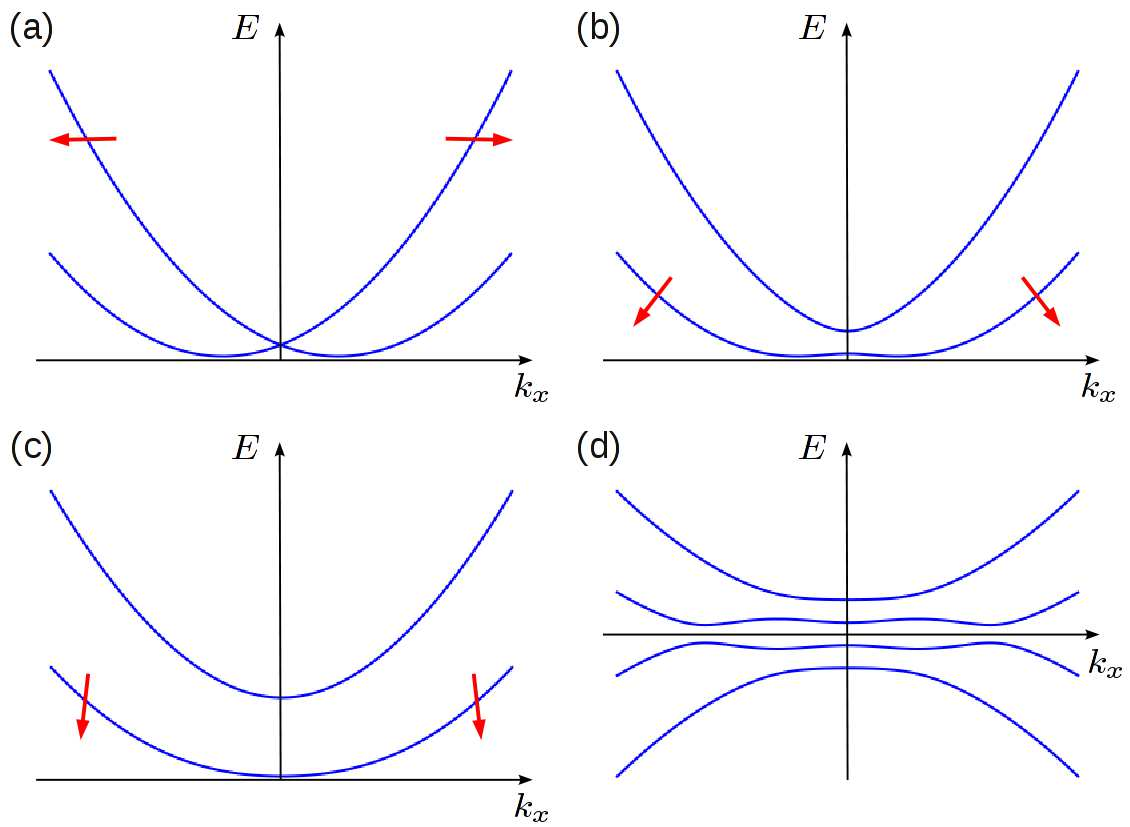
\includegraphics[height=0.78\textheight]{fig/ref/rys5.png}
  \zrodlo{\LF{} rys.~5: (a) $\tilde B=0$, (b) małe $\tilde B$, (c) duże $\tilde B$, (d) jak (c) z~$\Delta>0$ (BdG)}
\end{frame}

\end{document}
